\chapter{Methods}
\label{ch:methods}

\section{Methodology}

My methodological approach is cross-disciplinary and exploratory.
\todo{what disciplines??}
%
The cross-disciplinary aspect is inherent in the topic; it would
be impossible to characterise Indigenous seasons in this way without
integrating both qualitative and quantitative methods.
%
It is exploratory because there is no known precedent or published
method for quantification of an Australian Indigenous seasonal calendar.
This novelty means that the specific quantification methods used
were not known ahead of time, as they are informed and shaped by
interview data.  It also means that these methods themselves form
a novel contribution, which breaks ground for further research.

Project methods align with four distinct stages of the research:
\begin{enumerate}
\item Analysis of literature describing the Yolngu seasonal calendar
\item Interviews with Yolngu and non-Indigenous people who
    understand the Yolngu calendar
\item Quantitative analysis bridging literature and interview
    descriptions to the observational weather record, to characterise
    Yolngu seasons
\item Analysis of the derived seasonal record, such as typical
    conditions for each season and correlations with climate indices.
\end{enumerate}
These stages reflect the cross-disciplinary or mixed-methods approach,
with literature informing the direction of the research and qualitative
methods providing the framework for well-founded numerical analysis.


\paragraph{Qualitative research methodology} is particularly important
when working across cultures, for example when collaborating with
Indigenous people on western-style scientific research.
%
``Research'' is something of a dirty word in many Indigenous communities,
even where the people involved are trusted.  An experience of exploitation
or unequal benefits, where researchers come and go but leave nothing
for the Indigneous participants, remains too common \citep[eg.][]{smith1999}.

Without strong pre-existing relationships, in my case through several
years of engagment through the Uniting Church, this research would not
have been possible.  The trust earned through ongoing engagement allowed
me to commit to share my results and ensure that Yolngu participants will
also benefit from this study (see \cref{sec:applications-benefits}).  Without the introductions and logistical
assistance generously provided by the Uniting Church, it would have been impractical or
impossible to conduct such research for an Honours thesis.
%
In a letter inviting collaboration on this research (\cref{app:invitation-letter}),
a senior Yonlgu man explained that
\begin{quote} %{Rev. Garrawurra}
    For Yolngu (the people of North Eastern Arnhem Land) it is the Liyagadhaman
    who carry within them the wisdom and knowledge of these matters.
    It is right that in this research you have approached me to talk about these
    things. I can also introduce you to others who have this knowledge.
    ...
    Yolngu have made careful observation of the ways of nature and the seasons
    over the millennia and have passed on that knowledge down the generations.
    We know the changes that are taking place in the seasons and I am willing
    to talk with you about what I have seen happening around me.
\end{quote}


\paragraph{Data scoping} is a key influence on methodology.
What data is within scope or relvant to the research question --
and what isn't?
%
The decision should be principled and pragmatic.
The data must be sufficient for robust and well-founded analysis,
and it must also be possible to aquire and understand with limited
resources.  Secondary considerations include the potential applications
of the results, and avoiding undue difficulty for replication.

\todo{present options considered (ie past and future) and give reasons for rejection}

Interviews do not attempt to investigate historical understandings of
seasons or calendars, and are conducted in English -- linguistic study
is firmly out of scope.
%
Options for historical and projected weather data were considered, including
gridded reconstructions from observations, satellite datasets, and climate
model outputs (eg. CMIP5 or ACCESS).  Each of these failed to deliver the
required required detail, frequency, and variety of data required to detect
Yolngu seasons.  Direct weather observations provide a simple and robust basis
for the analysis, which focusses on the recent past.

All numerical weather data are drawn from daily direct observations at
surface weather stations (\cref{tab:weather-station-summary}).
Other datasets -- such as satellite observations or
climate models -- generally do not have both the spatial and the
temporal resolution required, or are missing key variables such as separate
surface wind vectors for morning and afternoon.
%
\defcitealias{BOM-data}{BOM 2016}
%
The Australian Bureau of Meteorology generously provided the data for each
weather station in the study area at no charge (included in the electronic appendices).
Similar data -- with the exception of wind -- is freely available online
for many weather stations \citepalias{BOM-data}, facilitating replication for other
calendars.


\paragraph{Context}
Context is important for this locally-based exploration of Yolngu seasons.
The townships of Galiwinku and Milingimbi are used as a case study for
practical reasons.  Personal connections and
logistical support from the Uniting Church facilitated fieldwork with limited
resources.  Yolngu seasons emphasise meteorological indicators, which allow
principled quantification based on the observational weather record.
%
The study area is on the north-east coast of the Northern Territory, shown
in  \cref{fig:arnhem-map}, about five hundred kilometers east of Darwin.
These sites fall within the Arnhem Coast bioregion.  The landscape is
dominated by tropical woodland, from mangroves on the coastline through
to dense forest to more open woody grasslands further inland \citep{ens2014}.


Qualitative seasonality is described for Galiwinku and Milingimbi;
quantitative weather observations from the neighboring communities of Waruwi, Maningrida, and Nhulunbuy
are also analysed.  Waruwi and Maningrida are in areas described by
other calendars, but provide a longer weather record in a similar climate
to the study area.
%
These stations were intended to provide validation data for a model fitted
to the Galiwinku and Milingimbi observations, as the record is too short to
split into training and validation sets temporally.  Analysis demonstrates
that Yolngu seasonal definitions are highly localised, and the seasonal
records from these stations are not usefully comparable.


\begin{figure}[t]
    \centering
    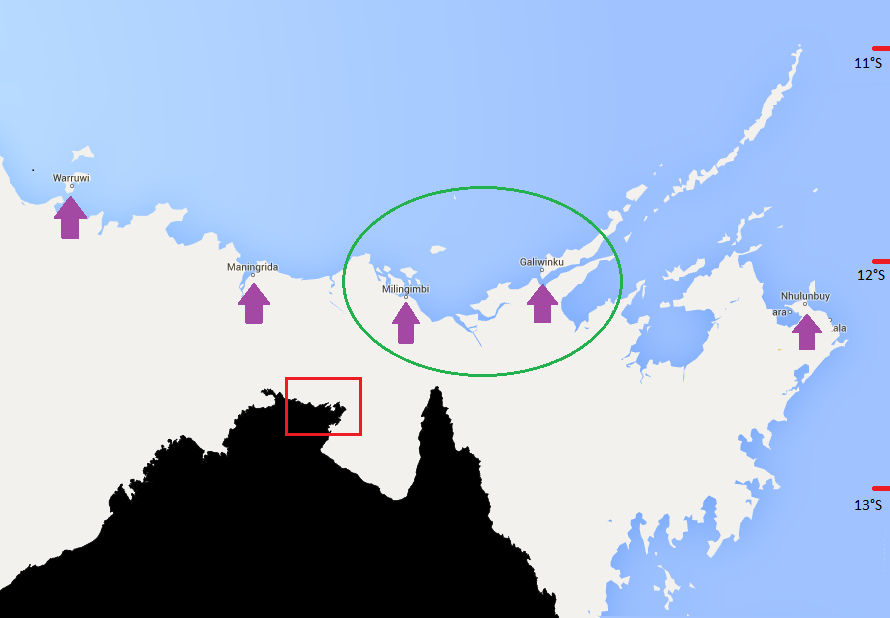
\includegraphics[width=\textwidth]{arnhem-map.png}
    \caption[Map of north-east Arnhem Land, showing the study area]{
        Map of north-east Arnhem Land, showing the study area, with inset silhouette
        of northern Australia showing map area (red box).  The five weather
        stations are located at airports serving the towns indicated by purple
        arrows.  The green oval highlights the region for which qualitiative
        data is collected.  Tick marks (east side) show latitude.}
    \label{fig:arnhem-map}
\end{figure}



\paragraph{Season recognition} is difficult to encode, and my methods can
best be described as exploratory.  The specifics are described in
\cref{sec:applying-seasons-method}, as they closely follow qualitative
findings and constitute a result in themselves.  Alternative approaches
which were tried and rejected are described in \cref{subsec:disc-season-detection}.

The general approach is to observe that seasons are recognised or defined
at least partially by weather conditions on a day-to-day basis.  It is
therefore possible to construct criteria for each season that describe
it in terms of daily weather observations, and derive a daily index for
each season.  Normalising these indices by z-score makes them directly
comparable, and the season with the greatest index on some day is said
to occur on that day.
%
Alternative approaches, such as definitions by trend change in weather
or onset thresholds, are not supported by the qualitative data.  See
\cref{ch:results} for details.


\paragraph{Quantitative} summaries are an important aspect of this
research, but do not form a key part of the scope and come at the
last stage of iterative methods.  This analysis is therefore
limited to the extent that it either informs comparisons with earlier work
or demonstrates potential for further study in a particular area.
In practice, this means calculating and plotting a small number of summary statistics
-- those which are meaningful for a complex calendar and supported by the
data.



\section{Qualitative and Interview Methods}

This research was approved by the ANU Human Research Ethics Committee,
as protocol \texttt{2015/543} on 06 October 2015.
Calendars and seasons are not usually considered secret business by Indigenous people, though
there may be particular sacred topics associated with them -- an explicit
invitation to come and learn minimises the risk of inappropriate sharing.
%
I rely on three sources of knowledge of and context for the Yolngu
seasons.  Interviews with Yolngu people form the basis of my qualitative
research, and are the definitive source of information about Yolngu seasons.
Interviews and discussion with non-Indigenous researchers or teachers with
experience in Yolngu communities contextualise this knowledge, and warn of
common misinterpretations - as well as pointing out nuances in the material.

The two primary sources are contextualised and supported by published
literature on cross-cultural research \citep[eg.][]{smith1999}, Australian
Indigenous seasons \citep[eg.][]{prober2011,oconnor2010}, and Yolngu seasons
\citep{davis1989,atlas2014}.  Secondary sources shape the specific methods
and interview questions (below).  Grey literature such as calendar posters
produced for remote schools and workbooks for cross-cultural teacher
training provided a starting point for informal conversations.


Prior to fieldwork, the planned sample was ten to twenty Yolngu people
of varied age and gender; interviews were to be conducted at Galiwinku
on Elcho Island, with supplementary interviews in Darwin.  Unfortunately
Rronang Garrawurra, who had offered his assistance with introductions
and accomodation (see \cref{app:invitation-letter}), was in Darwin due
to health issues and accomodation at Galiwinku was unavailable.
%
Fieldwork and interviews were conducted in Darwin.  Sample
recruitment followed a `snowball' pattern, where participants were asked
to suggest further potential participants \citep{patrick1996}.  The `seeds'
of this pattern were personal contacts in the Uniting Church and CSIRO
staff who worked on the Tropical Rivers and Coastal Knowledge project.
%
The final interview sample consisted of three older Yolngu men, four past
or practising teachers with several years experience in Arnhem Land, and
an experienced research team at CSIRO.  Most participants asked not to be identified, so comments
are not attributed to individuals.


I conducted a series of informal, semi-structured interviews discussing seasons
and climate, as avoidable paperwork or formalities tends to promote mutual
frustration rather than mutual learning when English may be a fourth language.
Thematic questions include:
\begin{itemize}
\item What are the names of the seasons?
\item When does [a season] usually occur?  How do you know when it starts (definition)?
\item How long does [a season] last?  What weather or events usually occur in this season?
\item Do you think the seasons have changed over your lifetime?  Why/why not?  How can you tell?
\item Are there some years where a season is skipped?  What happens?
\item Do you remember any unusual events?  What happened?
\item What might the calendar be like if [example climate impact] happened?
      (eg changes to wind, temperature, rainfall patterns)
\end{itemize}

Interviews generally took the form of participant-led discussion prompted
by one of the thematic questions.  The most consistently productive were
focussed on teaching about seasons: names and definitions, typical conditions
and timing, and extreme events or outliers.
%
These discussions took place in venues suggested by the participant, often
under a tree by the ocean, at a cafe, or in their home.  Each discussion
lasted between one and two hours, and I met with some participants multiple times
to discuss various aspects of Yolngu seasonality.

Just as Yolngu people offered their knowledge of seasons, discussions with
non-Indigenous people provided context and interpretative assistance as well
as their perspective on Yolngu seasons.  Immediate clarification and
feedback allowed for ongoing refinement of the questions, and pointed to
new directions or overlooked details which were elicited in subsequent
interviews.
%
Following the interviews, I also engaged in substantial reflection on the nature
of my questions and the ambiguity of the responses and data I collected.
In this process, allowing participants to discuss whatever they felt relevant
was a key way to remain open to unexpected information -- including insights
which changed my understanding of what a Yolngu seasonal calendar was.



\section{Application: from Qualitative to Numerical Data}

This research quantifies one Yolngu seasonal calendar, with six
seasons each year defined by weather conditions and events.
\cref{subsec:three-seasons-scales} provides a brief explanation of other
Yolngu seasonal calendars and justification of this scope.

\subsection{Weather Observations}
\label{ssec:weather-methods}

The key meteorological aspects of Arnhem Land seasonality are temperature,
rainfall, humidity, wind strength, and wind direction.  The annual
cycle is driven primarily by the Indian Ocean monsoon.  The climate is hot and
humid, with daytime temperatures between 25 and 40 degrees year-round.
%
This section describes the raw numerical data, quality checks, and handling of missing data.
The record begins with the installation of automatic weather stations
at several airports between 1990 and 2003, and continues to the present with only
minor gaps (where earlier observations exist they do not include all required
variables).  The results do not support
speculatation on the past or future state of Yolngu seasons.  The methods
however are applicable to data such as climate models, which provide
a clear direction for further work proposed in \cref{sec:further-study}.

\begin{table}[ht]
    \caption[List of weather stations providing data]{
        Summary description of weather stations used.
        Locations are visible in \cref{fig:arnhem-map}}
    \label{tab:weather-station-summary}
    \sffamily\small
    \centerline{
    \begin{tabular}{cllcccl}
        \toprule
        Station no.  &  Name                &  Location    &  Latitude  &  Longitude   &  Altitude  &  Opened   \\
        \midrule
        014401       &  Warruwi Airport     &  Warruwi     &  11.6500S  &  133.3797E   &  19m       &  Jan 1916 \\
        014404       &  Milingimbi Airport  &  Milingimbi  &  12.0932S  &  134.8919E   &  15m       &  Mar 2003 \\
        014405       &  Maningrida Airport  &  Maningrida  &  12.0569S  &  134.2339E   &  28m       &  Oct 2003 \\
        014508       &  Gove Airport        &  Nhulunbuy   &  12.2741S  &  136.8203E   &  52m       &  Jan 1944 \\
        014517       &  Ngayawili           &  Galiwinku   &  11.9971S  &  135.5726E   &  08m       &  Oct 1999 \\
        \bottomrule
    \end{tabular}
    }
\end{table}

\Cref{tab:weather-station-summary} shows the name, ID, and location of
the weather stations used.
%
The weather variables of interest are:
\begin{itemize}
\item Rainfall in the 24 hours before 9am (local time), in milimeters.
\item Maximum temperature in the 24 hours after 9am (local time), in Degrees C.
\item Minimum temperature in the 24 hours before 9am (local time), in Degrees C.
\item Humidity measured as average daily dew point temperature, in Degrees C.
\item Wind speed measured in kilometers per hour, at 9am and 3pm local time.
\item Wind direction recorded as 16 compass points, at 9am and 3pm local time.
\end{itemize}

Yolngu participants suggested that due to the effect of the sea breeze,
6pm would be more suitable than 3pm wind direction for season detection.
\Cref{fig:galiwinku-seabreeze-direction} shows wind direction by year
and day-of-year, as in \cref{fig:galiwinku-observations}.
%
Similar charts for wind speed and other stations are included in the electronic
appendices.  These charts show a northerly sea breeze, generally strong in the
noon, 3pm, and 6pm data.  Analysis and results are therefore based on the 3pm
wind data, which maintains consistency with the standard meteorological
afternoon and has longer record than 6pm at some stations.

The data are cleaned by discarding observations accumulated over multiple days.
Observations which have been quality-controlled by the BoM and are considered
`wrong', `suspect', or `inconsistent with other known information' are discarded.
Observations which have not been assessed are retained.
%
Missing data is not filled in any way, to convey the coverage of the record
and accurately represent missing data in the figures.  In scalar calculations,
missing data is propagated (eg ${NaN+10=NaN}$); in some aggregation
it is omitted from the sample (eg ${mean(1,NaN,5)=3}$, though
${mean(NaN,NaN)=NaN}$). Heatmap figures represent missing data as a black cell.


\subsection{Detection of Seasons}
\label{meth:seas-detection}

Seasons are detected at daily resolution, matching the input weather data.
Each of these methods assigns a confidence rating for each season to each day of
observations.  These ratings are then reconciled to a single season, or unknown,
for each day.  The reconciliation draws on participants' comments to drop inconsistent
ratings before comparing normalised season ratings.

For each season, I construct a set of boolean criteria based on participant
descriptions.  A raw index for each season is defined by
running these conditions over each day of data (giving True, False, or NaN),
and summing the values for each season for each day (giving NaN, 0, 1, ...).
\Cref{fig:season-definitions-code} shows the code used to build raw
seasonal indices.

Season-detection criteria can be defined in two ways: based on thresholds
in absolute measurement, or on trends.  Experimental analyses of trend-based
detection did not yield reliable results.  The threshold approach is more
practical and strongly grounded in qualitative season definitions, but both
wouuld merit investigation in future research.
%
Thresholds are set based on the calendar described in \cref{sec:calendar-description}.
For categorical criteria such as wind direction or the absence of rain days
they are reasonably rigorous; for quantitative criteria
such as ``very hot'', ``humid'', rain on ``most days'' or ``less frequently'',
rigour is more dificult.

The ideal solution would be to find a historical record of what season
it was on various days; regression analysis, (un)supervised classification,
or machine learning techniques could then associate seasons with typical
conditions.  Unfortunately, no such record exists -- in searching for one
I spoke to Yolngu people, current and ex-mission workers, CSIRO staff,
and academics from Charles Darwin University and Nungalinya College.
Future studies may wish to prioritise the ongoing creation of such a record,
for example via SMS surveys of Yolngu participants over one or more years.

Instead, I tried a range of values and selected those which appeared to
best reproduce the described timing of each season in the Galiwinku and
Milingimbi data.  This selection was on the basis of normalised season
indices before aggregation, so it tested for specific descriptions
rather than merely expected results.
%
This is probably the weakest step in the quantification method, but the data
required for more rigorous fitting of these parameters is not available.
Examination of figures for unfitted weather stations (see electronic appendices)
shows good agreement, suggesting that this method is sufficient for exploratory
analysis.

The final step normalises the index timeseries for each season by conversion to
a z-score, as the variation in data completeness and number of conditions between
seasons would not otherwise permit direct comparison between seasons.
This index is my representation of how well the season characterises that day's
conditions.  Aggregation of these indices is discussed in the next section.



\section{Quantitative Analysis}

All numeric tables and data visualisations in this thesis are produced
with Python scripts written by the author.  The raw data supplied by the
Bureau of Meteorology are supplied in the electronic appendices, as
are the analysis scripts.  This greatly facilitates reproduction of all
quantitative results and replication of the methods for other calendars
or datasets.  Running the scripts requires Python version 3.5 or later,
as well as the Pandas (0.18+) and Seaborn (0.7+) libraries with their
dependencies.

Seasons may occur multiple times in a given year in any order, as explained
in \cref{subsec:detection-advice}.  This presents a significant
challenge to reliable detection of seasonal onset, as respecting this
Indigenous interpretation of seasonality rules out
the simple approach of detecting an event and forward-filling the
associated season to the next detected event.  Instead, the research
uses a local analysis approach which seperately analyses each day of data,
smoothed with a short rolling mean.
%
The cost of this well-grounded system is increased `jitter', rapid
switching between seasons in periods when more than one is a close match
for conditions.  It is unknown to what extent this instability reflects Yolngu understandings.
%
Future studies may explore algorithms which represent a degree of path
dependence ('remembering' recent decisions), to account for Yolngu advice
that season change requires
several days observation.  This study prefers to avoid the risk of
over-fitting, sensitivity to initial conditions, and implementation
challenges such an approach brings.

In any case, Yolngu seasons cannot be well characterised by onset timing.
Instead of asking ``when does [this season] typically begin?'', which implies
that each season begins once per year, at a roughly constant date, a more
coherent question is to ask which season best matches conditions at a date,
or which is most commonly observed.
%
The benefits and drawbacks of various ways to characterise typical or onset
timing for seasons is discussed in \cref{subsec:disc-season-characterisation}.

